\documentclass[11pt,letterpaper]{article}
\usepackage[margin=2.5cm,top=3.5cm,bottom=3cm]{geometry}
\usepackage{booktabs}
\usepackage{graphicx}
\usepackage[hidelinks]{hyperref}
\usepackage{microtype}
\usepackage[table,dvipsnames]{xcolor}
\usepackage{longtable}
\usepackage{array}
\usepackage{caption}
\usepackage[T1]{fontenc}
\usepackage{lmodern}
\usepackage{fancyhdr}
\usepackage{amsmath}
\usepackage{titlesec}
\usepackage{enumitem}

\definecolor{wavblue}{RGB}{26,58,92}
\definecolor{wavgray}{RGB}{120,120,120}
\definecolor{wavlight}{RGB}{235,242,250}
\definecolor{wincolor}{RGB}{0,110,0}

\graphicspath{{/Users/egs/repos/waverider/benchmarks/canonical_tests/}}

\pagestyle{fancy}
\fancyhf{}
\fancyhead[L]{\small\color{wavgray}Manifold-Informed Architecture Benchmark \textemdash\ MNIST}
\fancyhead[R]{\small\color{wavgray}\texttt{waverider @ 4b8002e}}
\fancyfoot[C]{\small\color{wavgray}\thepage}
\renewcommand{\headrulewidth}{0.4pt}

\titleformat{\section}{\large\bfseries\color{wavblue}}{}{0em}{}[\color{wavblue}\titlerule]
\titleformat{\subsection}{\normalsize\bfseries\color{wavblue}}{}{0em}{}
\setlength{\parindent}{0pt}
\setlength{\parskip}{4pt plus 1pt}

\begin{document}

\begin{center}
  {\LARGE\bfseries\color{wavblue} Manifold-Informed Architecture Benchmark}\\[6pt]
  {\large MNIST: 10 classes, 784D input}\\[8pt]
  {\small Generated: 2026-04-14 20:54:27 \quad$|$\quad Apple M5 Max MacBook Pro, 64 GB RAM, 2TB SSD}\\[2pt]
  {\small\texttt{waverider @ 4b8002e} (--abbrev-re
4b8002ee9a2e3d56a219d7dab695a80b8efd1e07) \quad$|$\quad 2026-04-14 20:51:52 -0400}
\end{center}
{\color{wavblue}\noindent\rule{\linewidth}{1.5pt}}
\medskip

\noindent\colorbox{wavlight}{\parbox{\dimexpr\linewidth-2\fboxsep\relax}{
  \smallskip
  \textbf{Best:} Standard (128$\rightarrow$64)\quad test acc $= 0.9742 \pm 0.0010$\\[2pt]
  \textbf{Manifold:} 784D $\rightarrow$ 27D (96.6\%\ noise dimensions)\\[2pt]
  \smallskip
}}
\bigskip

\section{Experimental Setup}

\begin{tabular}{@{}ll@{}}
\toprule
\textbf{Parameter} & \textbf{Value} \\
\midrule
  Dataset & MNIST \\
  Input dimensionality & 784D \\
  Classes & 10 \\
  Intrinsic dim ($d$) & 27 \\
  Variance threshold ($\tau$) & 0.9 \\
  Epochs & 50 \\
  Trials & 5 \\
  Batch size & 128 \\
  Learning rate & 0.001 \\
  $k$ neighbors (local PCA) & 50 \\
\bottomrule
\end{tabular}

\section{Manifold Discovery}

Local PCA over the training set, $k = 50$ neighbors. Intrinsic dimensionality $d$ is taken as the maximum per-class maximum at $\tau = 0.9$, clamped to $n_{\mathrm{classes}} = 10$.

\begin{tabular}{@{}rrrrrr@{}}
\toprule
$\tau$ & Mean $d$ & Std & Min & Max & Noise (\%) \\
\midrule
  0.95 & 29.7 & 2.9 & 17 & 34 & 96.2 \\
  0.90 & 22.2 & 2.8 & 10 & 27 & 97.2 \\
  0.85 & 17.4 & 2.5 & 7 & 22 & 97.8 \\
  0.80 & 14.1 & 2.3 & 5 & 18 & 98.2 \\
\bottomrule
\end{tabular}

\subsection{Per-Class Intrinsic Dimensionality}

\begin{tabular}{@{}lrrrr@{}}
\toprule
Class & Mean $d$ & Std & Min & Max \\
\midrule
  Digit 8 & 24.8 & 1.0 & 23 & 27 \\
  Digit 3 & 24.2 & 1.5 & 18 & 26 \\
  Digit 5 & 23.8 & 2.0 & 16 & 27 \\
  Digit 4 & 23.3 & 1.1 & 20 & 25 \\
  Digit 2 & 23.0 & 3.4 & 7 & 27 \\
  Digit 0 & 22.9 & 1.4 & 18 & 25 \\
  Digit 9 & 20.6 & 2.0 & 12 & 23 \\
  Digit 6 & 20.6 & 2.9 & 6 & 24 \\
  Digit 7 & 19.2 & 2.8 & 11 & 23 \\
  Digit 1 & 16.9 & 1.5 & 13 & 20 \\
\bottomrule
\end{tabular}

\section{Architecture Comparison}

{\small
\begin{tabular}{@{}p{7cm}rccr@{}}
\toprule
\textbf{Architecture} & \textbf{Params} & \textbf{Test Acc ($\mu \pm \sigma$)} & \textbf{Loss} & \textbf{Acc/Kparam} \\
\midrule
  {Euclidean KNN (k=7)} & 0 & $0.8948 \pm 0.0000$ & --- & --- \\
  {ManifoldModel ($\tau$=0.9)} & 0 & $0.8958 \pm 0.0000$ & --- & --- \\
  {\color{wincolor}Standard (128$\rightarrow$64)\,$\star$} & 109,386 & $0.9742 \pm 0.0010$ & 0.3279 & 0.0089 \\
  {Wide Manifold (4d$\rightarrow$2d$\rightarrow$d, d=27)} & 92,431 & $0.9735 \pm 0.0012$ & 0.2989 & 0.0105 \\
  {Manifold (2d$\rightarrow$d, d=27)} & 44,155 & $0.9677 \pm 0.0006$ & 0.3700 & 0.0219 \\
  {PCA$\rightarrow$27D + MLP (2d$\rightarrow$d)} & 3,277 & $0.9623 \pm 0.0028$ & 0.1430 & 0.2937 \\
  {Intrinsic Dim (PCA$\rightarrow$27D$\rightarrow$output)} & 1,036 & $0.9511 \pm 0.0012$ & 0.1655 & 0.9181 \\
\bottomrule
\end{tabular}
}

\smallskip
{\small $\star$ = best performing architecture}

\section{Key Findings}

\begin{itemize}[leftmargin=*,itemsep=3pt]
  \item \textbf{Best architecture:} Standard (128$\rightarrow$64) \textemdash\ test accuracy $0.9742 \pm 0.0010$
  \item \textbf{Manifold compression:} 784D $\rightarrow$ 27D (96.6\%\ of ambient dimensions carry no structure)
\end{itemize}

\clearpage
\section{Result Figure}

\begin{figure}[htbp]
\centering
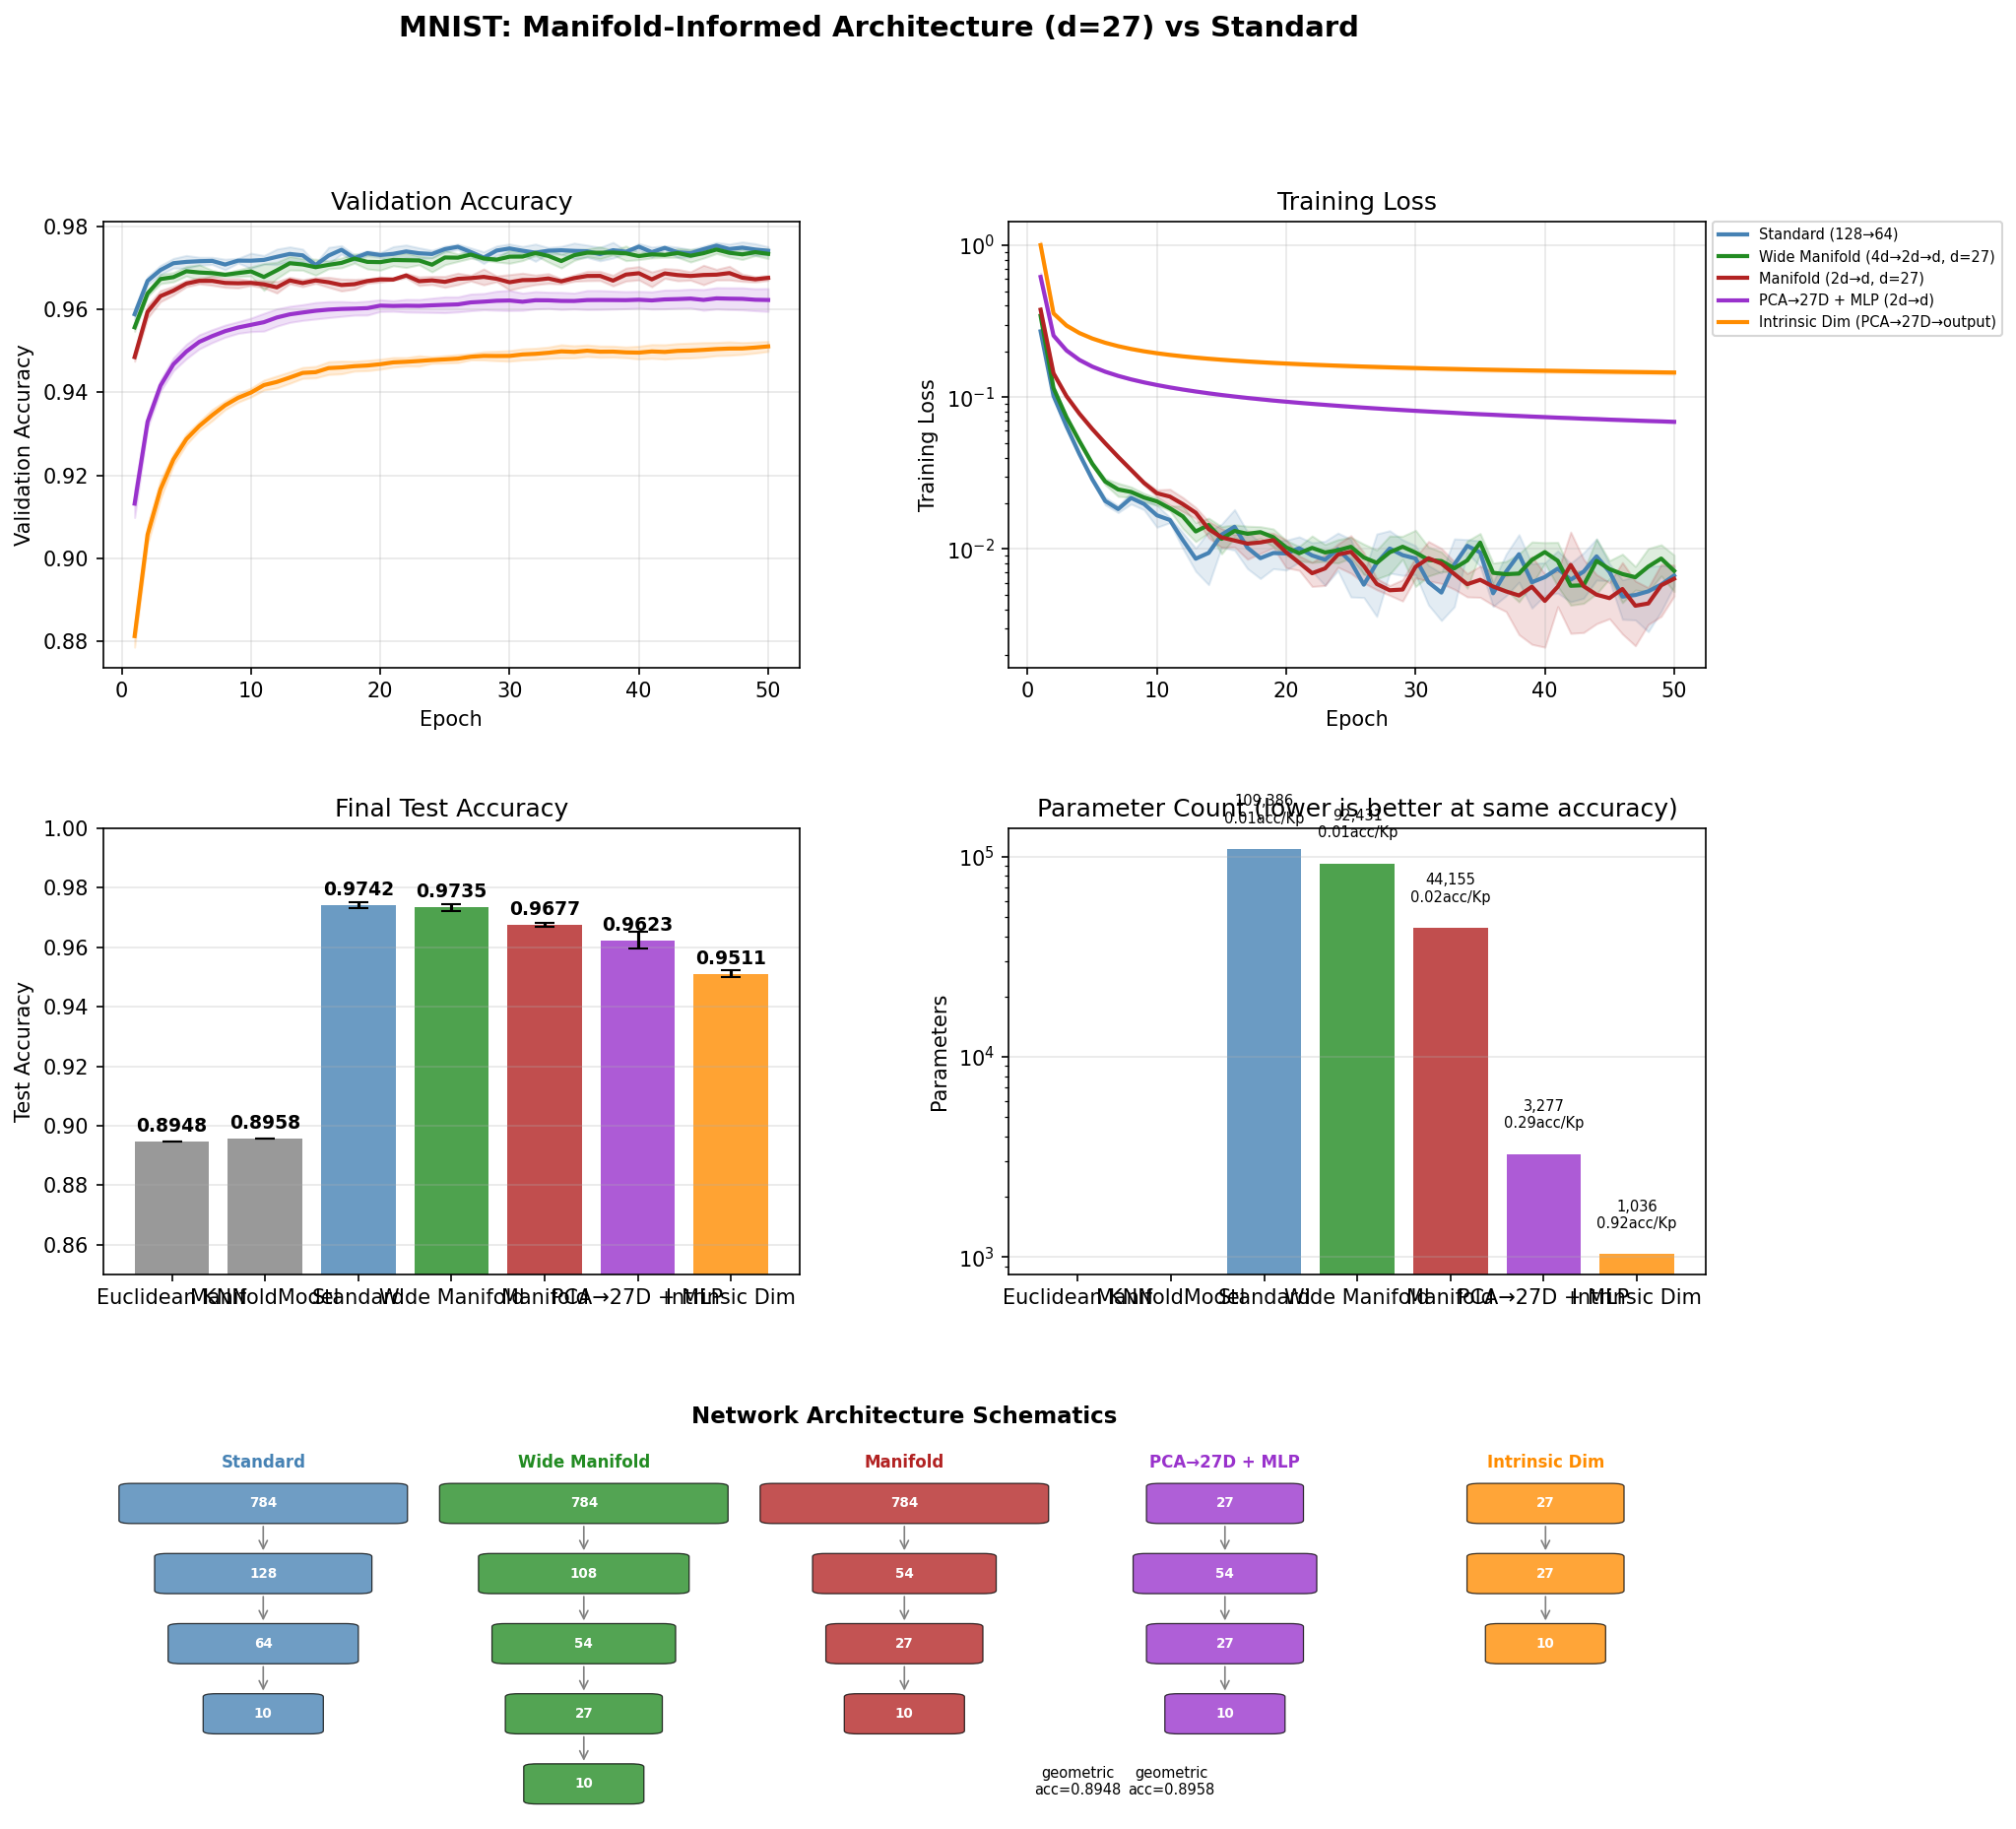
\includegraphics[width=\textwidth]{mnist_architecture_results}
\caption{MNIST manifold-informed vs.\ standard architecture comparison. $d = 27$, 50 epochs, 5 trials.}
\end{figure}

\section{Provenance}

\begin{tabular}{@{}ll@{}}
\toprule
\textbf{Item} & \textbf{Value} \\
\midrule
  Repository & \href{https://github.com/Flux-Frontiers/waverider}{Flux-Frontiers/waverider} \\
  Commit & \texttt{4b8002e} (--abbrev-re
4b8002ee9a2e3d56a219d7dab695a80b8efd1e07) \\
  Commit date & 2026-04-14 20:51:52 -0400 \\
  Commit message & add: cifar10 results \\
  Python & 3.12.13 \\
  TensorFlow & 2.16.2 \\
  Device & CPU (forced) \\
  Host & Turing \\
  OS & macOS-26.4-arm64-arm-64bit \\
  Machine & Apple M5 Max MacBook Pro, 64 GB RAM, 2TB SSD \\
  Generated & 2026-04-14 20:54:27 \\
\bottomrule
\end{tabular}

\end{document}
